%!TEX root = ./main.tex

% content goes here 
    
    \section{Git}
	\begin{frame}
		\frametitle{Git}
		% \framesubtitle{}
		\begin{columns}[c]
    		\column{.5\textwidth} 
        		\begin{itemize}
					\item Collaborate
                    \item Version Control
                    \item Open Source
          		\end{itemize}
          	\column{.5\textwidth}
            	\centering
				
\includegraphics[width=.7\linewidth,]{res/git}

				\vspace{1cm} % blank lines around this are needed

				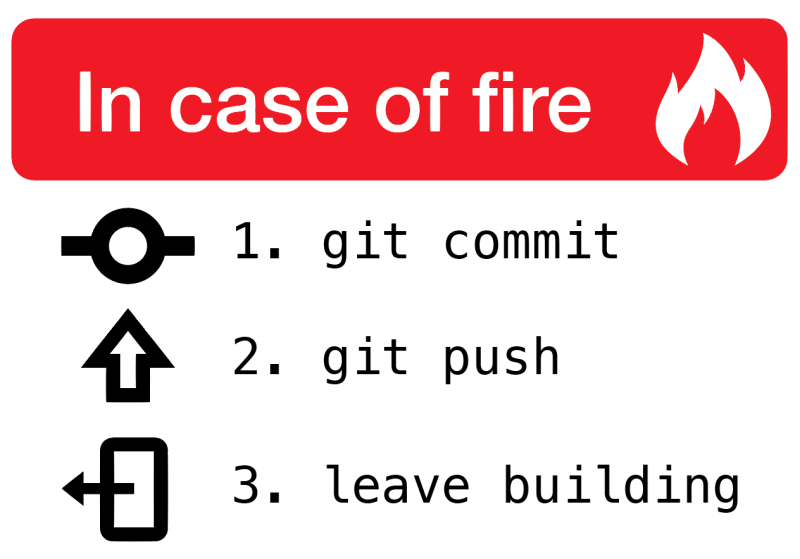
\includegraphics[width=.7\linewidth]{res/fire}
        \end{columns}
	\end{frame}
    
    \subsection{Workflow}
    \begin{frame}[allowframebreaks=10] % "=10" -> do not auto frame break
		\frametitle{Workflow}
		% \framesubtitle{}
        \begin{figure}
        	\centering
        	\includegraphics[width=0.8\linewidth]{"res/git_client-server"} \\
        \end{figure}
	\end{frame}
    
    \subsection{Demo}
    \begin{frame} 
		\frametitle{Demo}
        \begin{itemize}
        	\item Basic usage
            \item Merge conflicts
            \item exercise: 
            \href{https://classroom.github.com/g/8kE8ZX7m}{\textit{https://classroom.github.com/g/8kE8ZX7m}}
        \end{itemize}
	\end{frame}

	% end of content
